% Options for packages loaded elsewhere
\PassOptionsToPackage{unicode}{hyperref}
\PassOptionsToPackage{hyphens}{url}
%
\documentclass[
]{book}
\usepackage{amsmath,amssymb}
\usepackage{lmodern}
\usepackage{ifxetex,ifluatex}
\ifnum 0\ifxetex 1\fi\ifluatex 1\fi=0 % if pdftex
  \usepackage[T1]{fontenc}
  \usepackage[utf8]{inputenc}
  \usepackage{textcomp} % provide euro and other symbols
\else % if luatex or xetex
  \usepackage{unicode-math}
  \defaultfontfeatures{Scale=MatchLowercase}
  \defaultfontfeatures[\rmfamily]{Ligatures=TeX,Scale=1}
\fi
% Use upquote if available, for straight quotes in verbatim environments
\IfFileExists{upquote.sty}{\usepackage{upquote}}{}
\IfFileExists{microtype.sty}{% use microtype if available
  \usepackage[]{microtype}
  \UseMicrotypeSet[protrusion]{basicmath} % disable protrusion for tt fonts
}{}
\makeatletter
\@ifundefined{KOMAClassName}{% if non-KOMA class
  \IfFileExists{parskip.sty}{%
    \usepackage{parskip}
  }{% else
    \setlength{\parindent}{0pt}
    \setlength{\parskip}{6pt plus 2pt minus 1pt}}
}{% if KOMA class
  \KOMAoptions{parskip=half}}
\makeatother
\usepackage{xcolor}
\IfFileExists{xurl.sty}{\usepackage{xurl}}{} % add URL line breaks if available
\IfFileExists{bookmark.sty}{\usepackage{bookmark}}{\usepackage{hyperref}}
\hypersetup{
  pdftitle={Buenas prácticas para teléfonos quemados},
  pdfauthor={Elle Armageddon},
  hidelinks,
  pdfcreator={LaTeX via pandoc}}
\urlstyle{same} % disable monospaced font for URLs
\usepackage{longtable,booktabs,array}
\usepackage{calc} % for calculating minipage widths
% Correct order of tables after \paragraph or \subparagraph
\usepackage{etoolbox}
\makeatletter
\patchcmd\longtable{\par}{\if@noskipsec\mbox{}\fi\par}{}{}
\makeatother
% Allow footnotes in longtable head/foot
\IfFileExists{footnotehyper.sty}{\usepackage{footnotehyper}}{\usepackage{footnote}}
\makesavenoteenv{longtable}
\usepackage{graphicx}
\makeatletter
\def\maxwidth{\ifdim\Gin@nat@width>\linewidth\linewidth\else\Gin@nat@width\fi}
\def\maxheight{\ifdim\Gin@nat@height>\textheight\textheight\else\Gin@nat@height\fi}
\makeatother
% Scale images if necessary, so that they will not overflow the page
% margins by default, and it is still possible to overwrite the defaults
% using explicit options in \includegraphics[width, height, ...]{}
\setkeys{Gin}{width=\maxwidth,height=\maxheight,keepaspectratio}
% Set default figure placement to htbp
\makeatletter
\def\fps@figure{htbp}
\makeatother
\setlength{\emergencystretch}{3em} % prevent overfull lines
\providecommand{\tightlist}{%
  \setlength{\itemsep}{0pt}\setlength{\parskip}{0pt}}
\setcounter{secnumdepth}{5}
\usepackage{booktabs}
\ifluatex
  \usepackage{selnolig}  % disable illegal ligatures
\fi
\usepackage[]{natbib}
\bibliographystyle{apalike}

\title{Buenas prácticas para teléfonos quemados}
\author{Elle Armageddon}
\date{27-03-2017}

\begin{document}
\maketitle

{
\setcounter{tocdepth}{1}
\tableofcontents
}
\hypertarget{section}{%
\chapter*{}\label{section}}
\addcontentsline{toc}{chapter}{}

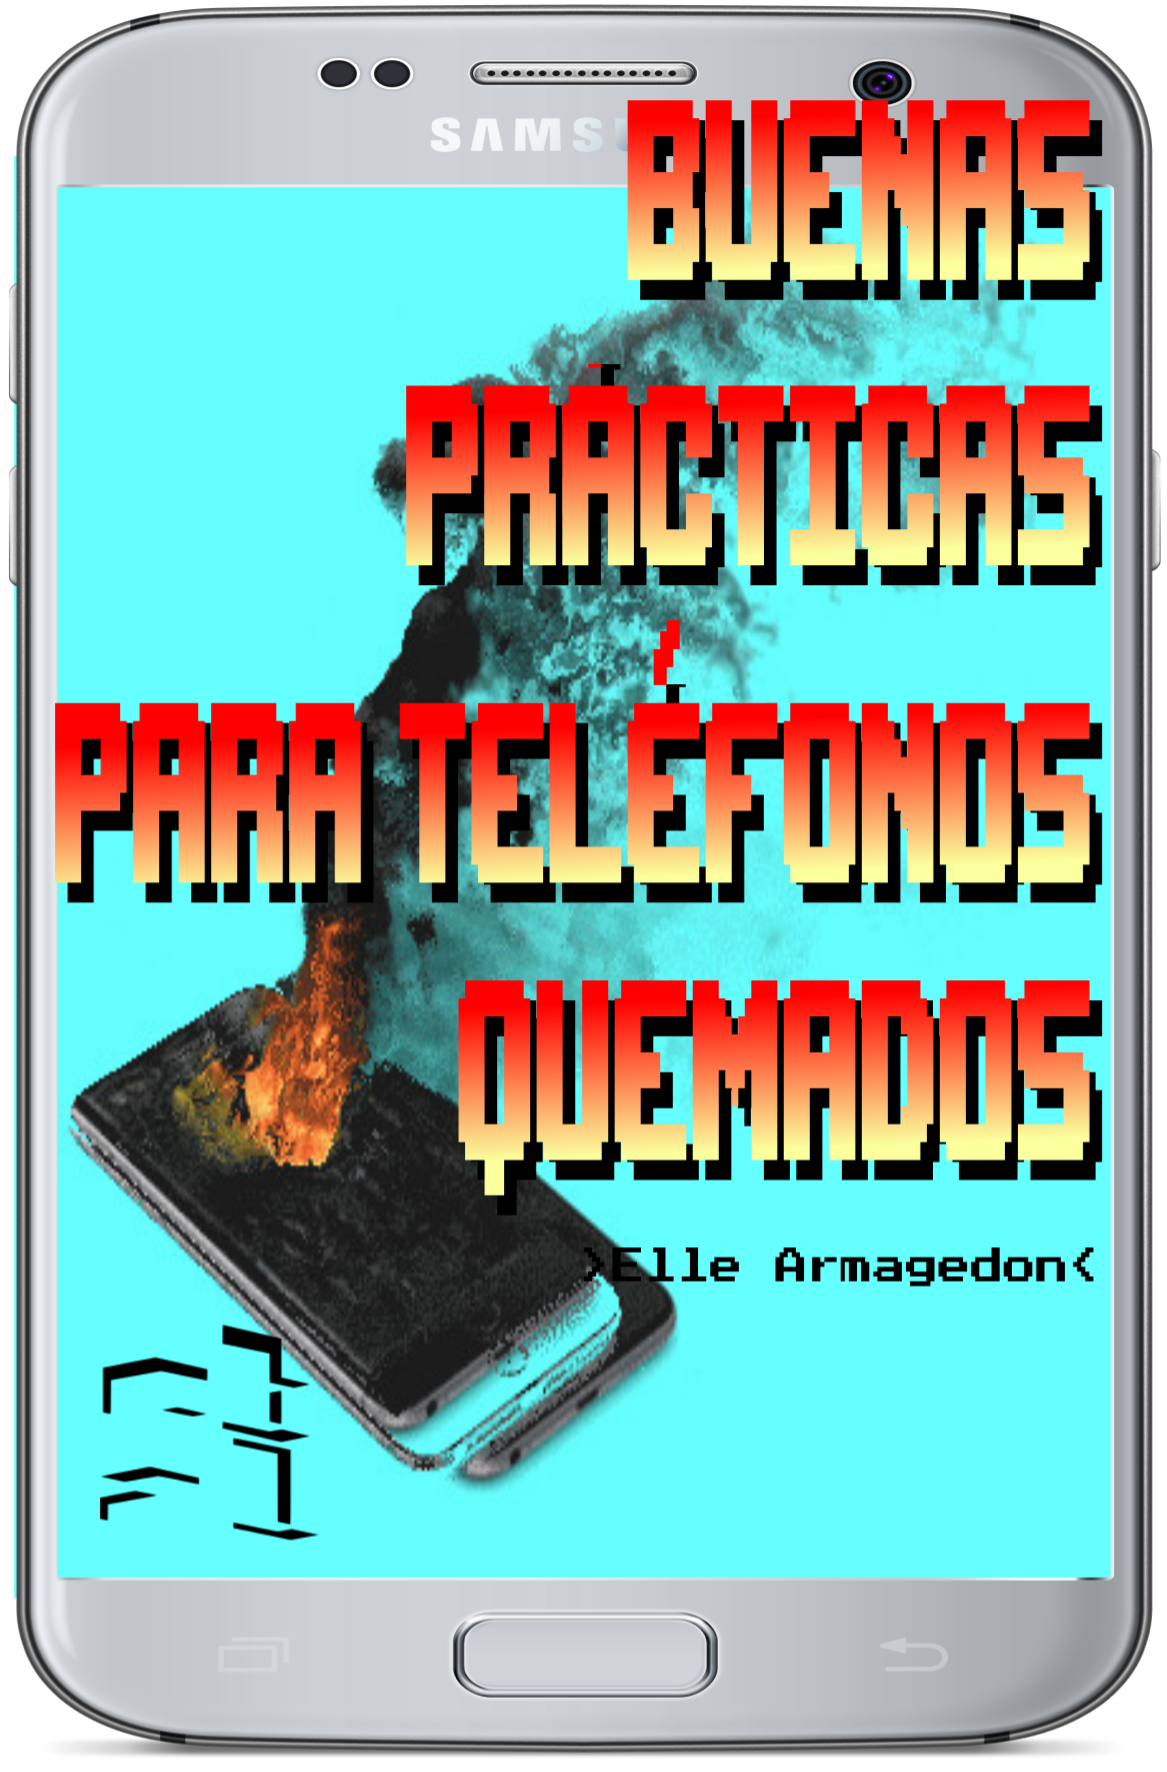
\includegraphics{images/cover2.png}

Armagedon, Elle

Buenas prácticas para teléfonos quemados / 1a ed.~- Ciudad Interdimensional de
Buenos Aires: etal, 2021.

Traducción: alf

Título original: \emph{Burner Phone Best Practices}.

\begin{figure}
\centering
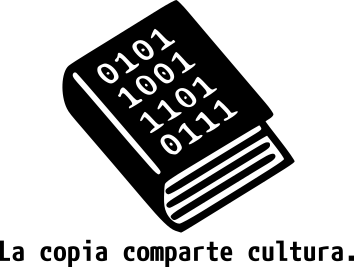
\includegraphics{images/lccc.png}
\caption{🄯2020 - etal
el texto de esta publicación y esta edición se liberan bajo la Licencia de
Producción de Pares}
\end{figure}

\hypertarget{licencia-de-producciuxf3n-de-pares-versiuxf3n-legible-por-humanes}{%
\chapter*{Licencia de Producción de Pares (Versión legible por humanes)}\label{licencia-de-producciuxf3n-de-pares-versiuxf3n-legible-por-humanes}}
\addcontentsline{toc}{chapter}{Licencia de Producción de Pares (Versión legible por humanes)}

\begin{quote}
Esto es un resumen legible por humanos del \href{http://endefensadelsl.org/ppl_es.html}{texto legal (la licencia
completa)}
\end{quote}

\hypertarget{ud.-es-libre-de}{%
\section*{Ud. es libre de}\label{ud.-es-libre-de}}
\addcontentsline{toc}{section}{Ud. es libre de}

\begin{itemize}
\tightlist
\item
  Compartir - copiar, distribuir, ejecutar y comunicar públicamente la obra
\item
  Hacer obras derivadas
\end{itemize}

\hypertarget{bajo-las-condiciones-siguientes}{%
\section*{Bajo las condiciones siguientes:}\label{bajo-las-condiciones-siguientes}}
\addcontentsline{toc}{section}{Bajo las condiciones siguientes:}

\begin{figure}
\centering

\includegraphics{images/by.png}
\caption{\textbf{Atribución} - Debe reconocer los créditos de la obra de la manera
especificada por el autor o el licenciante (pero no de una manera que sugiera
que tiene su apoyo o que apoyan el uso que hace de su obra).}
\end{figure}

\begin{figure}
\centering

\includegraphics{images/sa.png}
\caption{\textbf{Compartir bajo la Misma Licencia} - Si altera o transforma esta obra, o
genera una obra derivada, sólo puede distribuir la obra generada bajo una
licencia idéntica a ésta.}
\end{figure}

\begin{figure}
\centering

\includegraphics{images/nc.png}
\caption{\textbf{No Capitalista} - La explotación comercial de esta obra sólo está permitida
a cooperativas, organizaciones y colectivos sin fines de lucro, a
organizaciones de trabajadores autogestionados, y donde no existan relaciones
de explotación. Todo excedente o plusvalía obtenidos por el ejercicio de los
derechos concedidos por esta Licencia sobre la Obra deben ser distribuidos por y
entre los trabajadores.}
\end{figure}

\hypertarget{entendiendo-que}{%
\section*{Entendiendo que}\label{entendiendo-que}}
\addcontentsline{toc}{section}{Entendiendo que}

\begin{itemize}
\item
  \textbf{Renuncia} - Alguna de estas condiciones puede no aplicarse si se obtiene
  el permiso del titular de los derechos de autor.
\item
  \textbf{Dominio Público} - Cuando la obra o alguno de sus elementos se halle en
  el dominio público según la ley vigente aplicable, esta situación no quedará
  afectada por la licencia.
\item
  \textbf{Otros derechos} - Los derechos siguientes no quedan afectados por
  la licencia de ninguna manera:

  \begin{itemize}
  \item
    Los derechos derivados de usos legítimos u otras limitaciones
    reconocidas por ley no se ven afectados por lo anterior;
  \item
    Los derechos morales del autor;
  \item
    Derechos que pueden ostentar otras personas sobre la propia obra o
    su uso, como por ejemplo derechos de imagen o de privacidad.
  \end{itemize}
\item
  \textbf{Aviso} - Al reutilizar o distribuir la obra, tiene que dejar muy en claro
  los términos de la licencia de esta obra. La mejor forma de hacerlo es
  enlazar a esta página.
\end{itemize}

\hypertarget{una-guuxeda-de-usuarie}{%
\chapter*{1.- Una guía de usuarie}\label{una-guuxeda-de-usuarie}}
\addcontentsline{toc}{chapter}{1.- Una guía de usuarie}

Un teléfono quemado es un teléfono para un solo uso, no vinculado a tu identidad, que teóricamente puede usarse para comunicarse de forma anónima en situaciones en las que las comunicaciones pueden ser monitoreadas. Si el uso de un teléfono quemado es en sí una ``mejor práctica'' es un tema de debate, pero si elegiste usar uno, hay varias cosas que tenés que tener en cuenta.

\hypertarget{los-teluxe9fonos-quemados-no-son-teluxe9fonos-descartables}{%
\chapter*{2.- Los teléfonos quemados no son teléfonos descartables}\label{los-teluxe9fonos-quemados-no-son-teluxe9fonos-descartables}}
\addcontentsline{toc}{chapter}{2.- Los teléfonos quemados no son teléfonos descartables}

Un teléfono quemado es, como se mencionó anteriormente, un teléfono para un solo uso y adquirido específicamente para comunicaciones anónimas. Se considera un medio de comunicación clandestino y su eficacia se basa en aportar a tener prácticas de seguridad robustas. Un teléfono descartable es aquel que comprás y usás normalmente contemplando la posibilidad de que pueda perderse o romperse.

\hypertarget{un-quemado-sirve-para-comunicarse-solamente-con-quemados}{%
\chapter*{3.- Un quemado sirve para comunicarse solamente con quemados}\label{un-quemado-sirve-para-comunicarse-solamente-con-quemados}}
\addcontentsline{toc}{chapter}{3.- Un quemado sirve para comunicarse solamente con quemados}

El uso de un teléfono quemado para hablar con el teléfono cotidiano de otra persona deja un rastro entre vos y tu contacto. Para la garantizar la privacidad de las personas dentro de tu círculo de comunicación, los teléfonos quemados solo deben usarse para comunicarse con otros teléfonos quemados, de modo que tus relaciones no comprometan tu privacidad. Hay varias formas de organizar esto, pero probablemente lo mejor sea memorizar tu propio número y compartirlo en persona con quien quieras comunicarte. Acuerden de antemano un modelo de mensaje de texto arquetípico, de modo que cuando enciendas tu teléfono puedas identificar a quien pertenece en función del mensaje y nada más. En situaciones en las que te encuentres con gente en una gran multitud, probablemente también esté bien completar este proceso con el teléfono encendido. En cualquier caso, no es necesario responder al mensaje de iniciación a menos que tengas información importante para compartir. Acordate también que es preferible que mantengas tus contactos y tus comunicaciones lo más dispersas posible, a fin de minimizar la exposición.

\hypertarget{nunca-prendas-un-teluxe9fono-quemado-en-tu-casa}{%
\chapter*{4.- Nunca prendas un teléfono quemado en tu casa}\label{nunca-prendas-un-teluxe9fono-quemado-en-tu-casa}}
\addcontentsline{toc}{chapter}{4.- Nunca prendas un teléfono quemado en tu casa}

Dado que los teléfonos celulares registran y transmiten datos de ubicación, nunca deberías encender un teléfono quemado en algún lugar al que puedas quedar vinculade. Obviamente, esto se refiere a tu casa, pero también es extensible a las casas de tus amigues, compañeres, tu lugar de trabajo, tu escuela, gimnasio y cualquier otro lugar que visites con regularidad.

\hypertarget{nunca-prendas-un-teluxe9fono-quemado-cerca-de-tu-teluxe9fono-principal}{%
\chapter*{5.- Nunca prendas un teléfono quemado cerca de tu teléfono principal}\label{nunca-prendas-un-teluxe9fono-quemado-cerca-de-tu-teluxe9fono-principal}}
\addcontentsline{toc}{chapter}{5.- Nunca prendas un teléfono quemado cerca de tu teléfono principal}

Como se explicó anteriormente, los teléfonos celulares son básicamente dispositivos de seguimiento con funciones y características adicionales relativamente interesantes. Debido a esto, nunca deberías encender un teléfono quemado cerca de tu teléfono ``real''. Dejar un rastro de datos que coloque tu teléfono quemado en el mismo lugar y al mismo tiempo que tu teléfono de identificación personal es una manera de que ambos teléfonos queden vinculados. Esto también significa que, a menos que estés rodeade por una multitud, no deberías encender tu teléfono quemado cerca de los teléfonos quemados encendidos de tus contactos.

\hypertarget{no-te-refieras-a-otres-ni-a-vos-misme-por-sus-nombres-personales}{%
\chapter*{6.- No te refieras a otres ni a vos misme por sus nombres personales}\label{no-te-refieras-a-otres-ni-a-vos-misme-por-sus-nombres-personales}}
\addcontentsline{toc}{chapter}{6.- No te refieras a otres ni a vos misme por sus nombres personales}

Dado que el propósito de usar un teléfono quemado es preservar tu anonimato y el anonimato de las personas que te rodean, cualquier práctica que en el uso de ese teléfono, te identifique a vos o a algune de tus contactos, ya sea mencionando nombres o cualquier tipo de información personal, socava dicho objetivo. Por eso, es recomendable que no uses el nombre legal de nadie cuando te comuniques a través de un teléfono quemado, y preferentemente tampoco uses ningún tipo de seudónimo. Si es imperativo usar identificadores, es conveniente que sean únicos, establecidos con anticipación y no se reutilicen.

Considerá usar una frase a modo de contraseña para comunicarte, en lugar de usar nombres. Esto también permite la llamada y respuesta como autenticación. Por ejemplo, te da la certeza de que el contacto con el que deseás comunicarte es el contacto correcto si responde a su de forma correcta. Además, esta práctica de autenticación permite el uso de un código de coacción que se puede usar si la persona con la que estás tratando de coordinar necesita ayuda.

\hypertarget{cuidado-con-los-imsi-catchers}{%
\chapter*{7.- Cuidado con los IMSI catchers}\label{cuidado-con-los-imsi-catchers}}
\addcontentsline{toc}{chapter}{7.- Cuidado con los IMSI catchers}

Una razón por la que es deseable mantener tus frases de autenticación y
coacción lo más crípticas posible es porque las agencias de aplicación de la
ley de todo el mundo utilizan receptores de identidad de suscriptor móvil
(IMSI catchers), también conocidos como ``mantarrayas'' o ``simuladores de
sitios móviles'' para capturar mensajes de texto y llamadas telefónicas dentro
de ciertos rangos de distancia. Estos dispositivos pretenden ser torres de
telefonía móvil, interceptan y registran tus comunicaciones y luego las pasan
a torres de telefonía móvil reales para que tus contactos previstos también las
reciban. Debido a esto, probablemente no quieras usar tu quemado para enviar
mensajes de texto como, ``Ey, ¿estás en la protesta?'' o ``¿Trajiste las
Molotov?''.

En circunstancias normales el uso de servicios mensajería cifrada como
Signal puede eludir el uso de Stingrays con bastante eficacia, pero como los
teléfonos quemados no suelen tener la capacidad de enviar mensajes cifrados
(a menos que estés comprando teléfonos inteligentes quemados), hay que
tener cuidado sobre lo que se dice.

\hypertarget{los-teluxe9fonos-quemados-son-para-un-solo-uso}{%
\chapter*{8.- Los teléfonos quemados son para un solo uso}\label{los-teluxe9fonos-quemados-son-para-un-solo-uso}}
\addcontentsline{toc}{chapter}{8.- Los teléfonos quemados son para un solo uso}

Los teléfonos quemados están diseñados para usarse una vez y luego se consideran ``quemados''. Hay muchas razones para esto, pero la razón principal es que por lo general no es deseable que nuestras acciones clandestinas estén vinculadas. Si el mismo teléfono quemado comienza a aparecer en los mismos eventos, las personas que investigan esos eventos tienen un conjunto más amplio de datos para crear perfiles. Lo que esto significa es que, si lo que estás haciendo realmente requiere un teléfono quemado, entonces lo que estás haciendo requiere un quemado nuevo cada vez. En general, hay que evitar que la ejecución descuidada de las medidas de seguridad anule todos tus esfuerzos.

\hypertarget{adquiruxed-tu-teluxe9fono-quemado-con-cuidado}{%
\chapter*{9.- Adquirí tu teléfono quemado con cuidado}\label{adquiruxed-tu-teluxe9fono-quemado-con-cuidado}}
\addcontentsline{toc}{chapter}{9.- Adquirí tu teléfono quemado con cuidado}

Para que tu quemado sea imposible de rastrear es preferible que lo pagues en efectivo; es decir que no se use tarjeta de débito para efectuar el pago. Y preguntarse: ¿hay cámaras de vigilancia en el lugar donde lo compra o en sus alrededores? No lleves tu teléfono personal al lugar donde compres tu quemado. Considerá caminar o ir en bicicleta hasta el lugar de la compra; cubriendo rasgos fácilmente identificables con ropa o maquillaje; y en lo posible, tratá de no comprar un quemado en un lugar que frecuentes con suficiente regularidad.

\hypertarget{nunca-asumas-que-los-teluxe9fonos-quemados-son-seguros}{%
\chapter*{10.- Nunca asumas que los teléfonos quemados son ``seguros''}\label{nunca-asumas-que-los-teluxe9fonos-quemados-son-seguros}}
\addcontentsline{toc}{chapter}{10.- Nunca asumas que los teléfonos quemados son ``seguros''}

Para que los teléfonos quemados preserven su privacidad todes les involucrades en el círculo de comunicación deben mantener y compartir una política común de cuidados. El uso anónimo de los quemados exige precauciones adecuadas y prácticas de cuidados por parte de todes en la red: una falla de una persona puede comprometer a todes. En consecuencia, es importante tanto asegurarse de que todas las personas con las que te estés comunicando estén en sintonía con respecto al uso anónimo y adecuado de los teléfonos quemados, como también asumir que es probable que alguien sea descuidade. Ésta es otra buena razón para tener cuidado con tus comunicaciones incluso cuando utilices teléfonos quemados. Siempre asumí la responsabilidad de garantizar los cuidados que ello implica y no dudes en borrar y deshacerte de su quemado cuando sea necesario.

  \bibliography{book.bib,packages.bib}

\end{document}
